\documentclass[../main]{subfiles}
\ifSubfilesClassLoaded{
    \dominitoc
    \tableofcontentsfile
	\pagenumbering{arabic}
    \setcounter{page}{1}
}{}

\begin{document}
\graphicspath{{06-Analyse/figures},{../06-Analyse/figures}, {../06b-Analyse-2D}}

\chapter{Extension aux cartes en deux dimensions}

\minitoc
Nous avons étudié des comportements de base de cartes 1D sur des données en une dimension. 
Cependant, les cartes auto-organisatrices utilisées en pratique sont des cartes en deux dimensions, qui permettent bien mieux de cartographier des données en grande dimension.
Ce chapitre présente une étude préliminaire d'architectures de deux et trois cartes en deux dimensions. Nous étudierons si les mécanismes d'organisation observés sur des cartes 1D se retrouvent sur des cartes 2D, et chercherons à identifier les limites et perspectives du passage 1D à 2D.

\section{Jeu d'entrées géométriques}

Nous travaillons à présent sur des cartes prenant chacune des entrées en deux dimensions.
Pour analyser un cas géométrique similaire au cas en une dimension, les entrées multimodales sont donc ici des points en 4 dimensions pour une structure de 2 cartes, 6 dimensions pour 3 cartes. 
Ces points sont situés sur une sphère en 3D dont on a effectuée une rotation dans l'espace 4D, de la même façon que les entrées en 3D se trouvaient sur un cercle 2D dont on a effectué une rotation dans l'espace, voir figure~\ref{fig:sphere_inputs}. 
La variable $U$ paramétrant cette surface est alors en deux dimensions et permet de représenter le modèle d'entrées.
Nous normalisons les entrées entre 0 et 1 sur chaque dimension, entrainant une légère déformation de la sphère.

Nous considérons d'abord une architecture de deux cartes en une dimension. Chaque carte possède une couche de poids externes  $\w\ext \in [0,1]^2$ et une couche de poids contextuels $\w_c \in [0,1]^2$. Les BMUs de chaque cartes sont maintenant représentés par des positions en deux dimensions $\bmu = (\bmu_0, \bmu_1)$. Nous prenons des cartes  de taille $100x100$.

\begin{figure}
	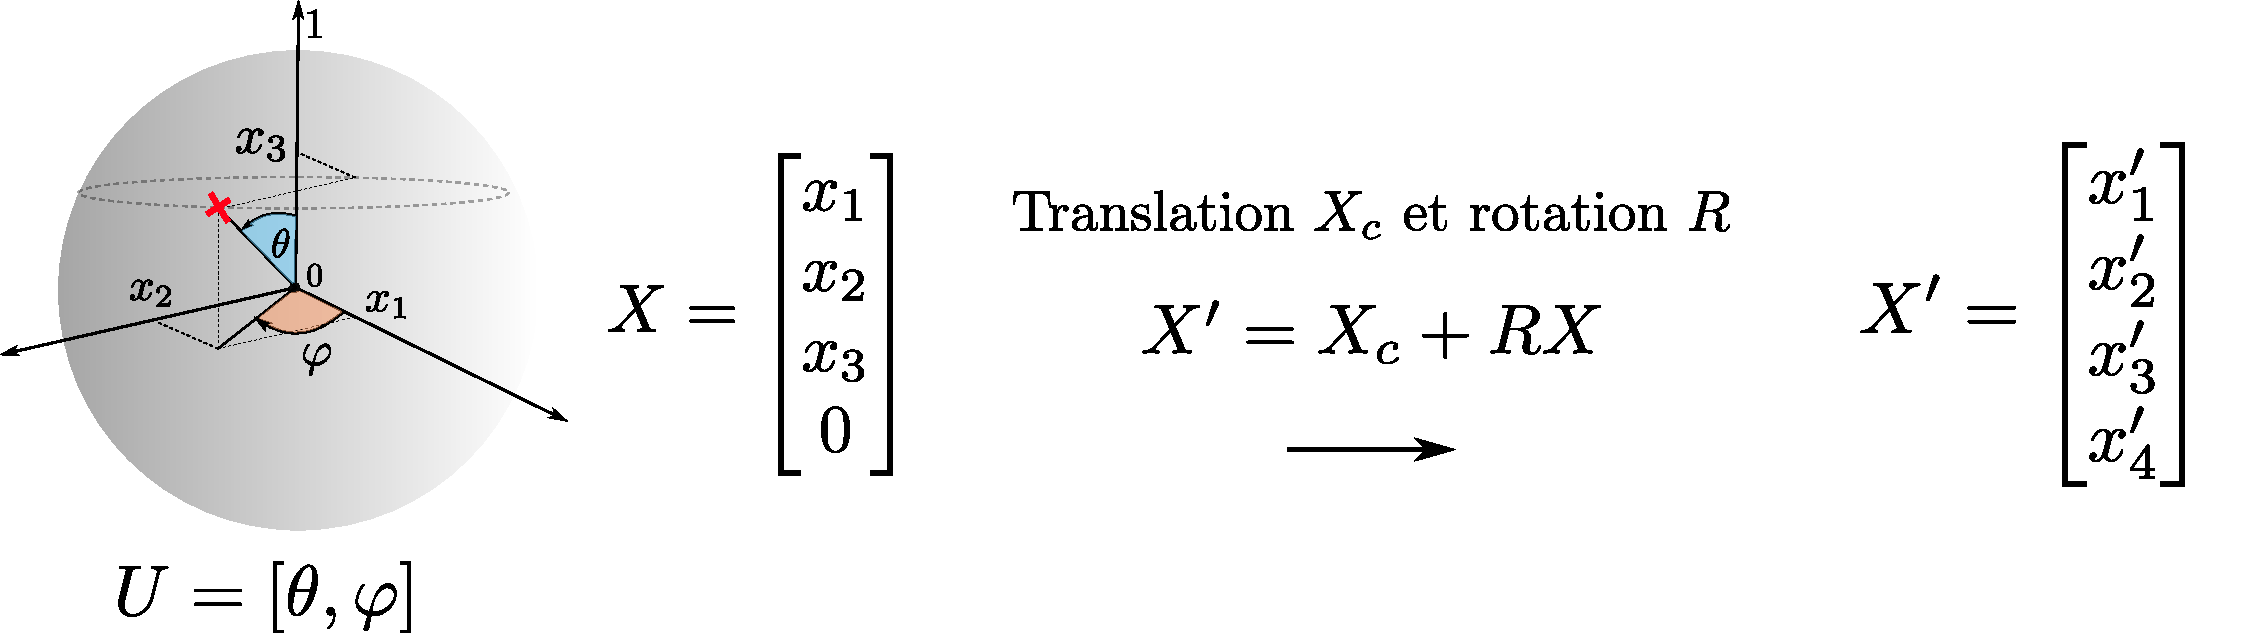
\includegraphics[width=\textwidth]{sphere_inputs.pdf}
	\caption{Transformation d'une surface d'un espace 3D en surface dans un espace 4D ou 6D. Les points restent positionnés sur une surface, mais sont plongés dans un espace de plus grande dimension. La rotation permet de répartir les coordonnées des points sur les dimensions. \label{fig:sphere_inputs}}
\end{figure}

\section{Organisation des poids}

Une première difficulté apportée par les deux dimensions est que l'organisation des poids externes n'est pas forcément assurée pour un rayon de voisinage constant, même dans une carte sans connexions contextuelles. Par exemple, l'organisation attendue d'une carte sur le carré $[0,1]^2$ est que les coins de la carte viennent dans les coins du carré. Cependant, les mécanismes d'organisation peuvent conduire à une carte tordue en son milieu, par exemple en \label{fig:torsion}.

\begin{figure}
	\centering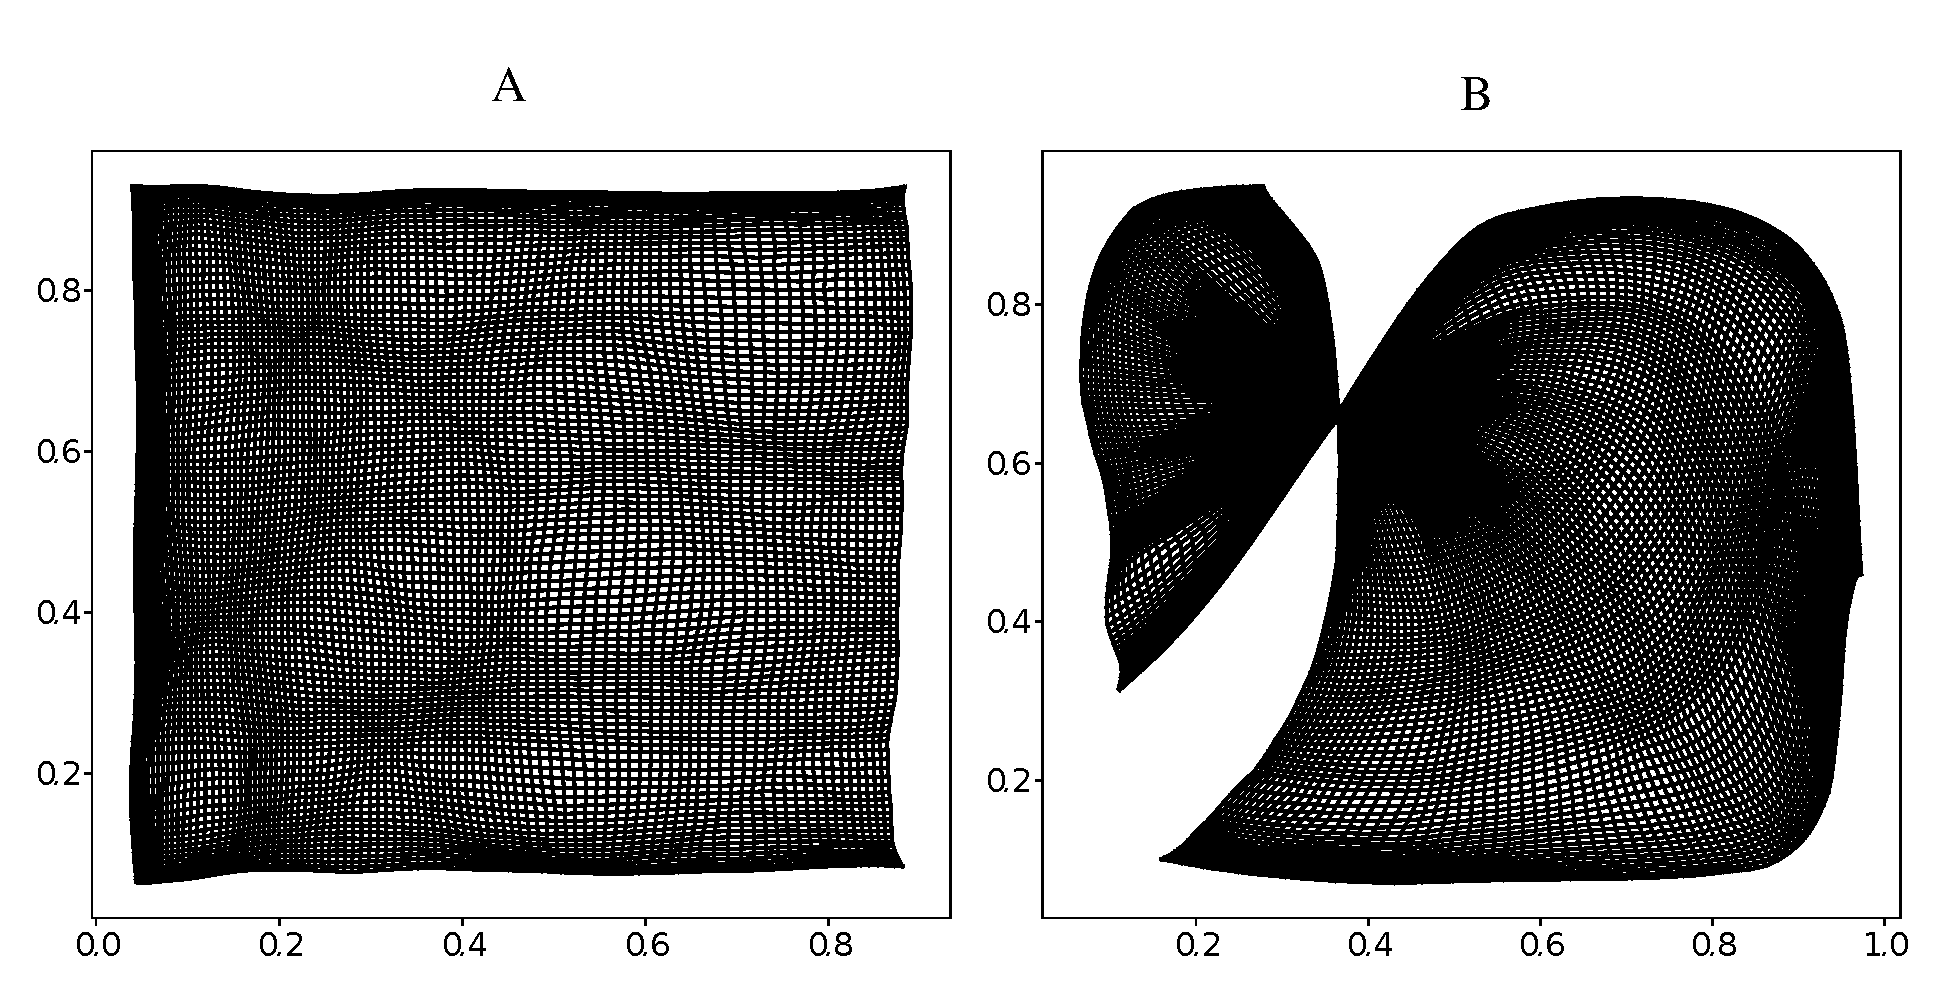
\includegraphics[width=0.7\textwidth]{we_cub_example.pdf}
	\caption{Exemple de point de torsion dans une carte 2D dépliée sur des entrées dans $[0,1]^2$ (B). La carte A au contraire est bien dépliée~: deux entrées proches sont représentées par des BMUs proches. Cette disposition présentant un point de torsion peut évoluer vers une carte bien dépliée ou vers un état stable présentant un point de torsion, en fonction des paramètres d'apprentissage. \label{fig:torsion}
	}
\end{figure}

Dans une architecture CxSOM, cela peut poser un problème pour l'utilisation de la position du BMU en tant que représentation de l'entrée~: la position du BMU n'est plus directement représentative de l'entrée. Deux entrées proches peuvent avoir leur BMU de chaque côté de la carte.
Dans un premier temps, nous avons choisi de forcer les cartes à bien se déplier . Pour cela, nous laissons les poids externes s'organiser sur quelques centaines d'itérations, préalablement aux poids contextuels, en prenant un grand rayon de voisinage $r_e = 0.5$. 
Ce grand rayon permet d'éviter les zones de torsion dans la carte. Après cette étape préalable, nous réduisons le rayon externe  à $r_e = 0.2$ et effectuons l'apprentissage des poids externes et contextuels comme décrit dans le modèle CxSOM. Les poids externes affinent alors leur apprentissage et les poids contextuels s'organisent sur une carte "bien dépliée". 
La généralisation de l'organisation des architectures 2D serait à explorer pour assurer une robustesse de l'algorithme sur des données quelconques~: il est en effet compliqué de s'assurer du bon dépliement d'une carte en pratique sur des données de grande dimension.

\subsection{Organisation de cartes sur des entrées indépendantes}

Intéressons nous d'abord à l'organisation d'une architecture de deux cartes, prenant des entrées $\inpx\m{1}, \inpx\m{2} \in [0,1]^2 \times 0,1]^2$. Les entrées sont indépendantes. Nous prenons des rayons de voisinage $r_e = 0.2, r_c = 0.05$.
Dans l'architectures de cartes 1D, l'apprentissage sur des données indépendantes conduit à la formation de zones dans les poids contextuels de chaque carte. Nous voulons vérifier si la présence de telles zones est observable sur des cartes 2D.

Nous nous intéressons d'abord aux motifs formés par les poids externes et contextuels sur chaque carte.

En Figure~\ref{fig:2som_cub_we}~, nous traçons les poids externes des cartes dans l'espace des entrées~: chaque point $p$ de la carte est positionné en $\w_e(p)$ et relié à ses voisins pour représenter le voisinage.

Nous utilisons une représentation à l'aide d'une carte de coloration pour les poids contextuels en figure~\ref{fig:2som_cub_wc}. Le pixel situé à la position $p$ sur l'image prend la couleur correspondant à la valeur de son poids contextuel $w_c$, définie par la carte de coloration tracée à droite sur la figure.
Cette représentation permet de faire apparaître clairement des motifs dans la disposition des poids.
Tracer les poids nous permet ici de comparer l'organisation d'une carte à celle observée en une dimension. Nous soulignons cependant que cette représentation ne permet pas de détecter quelles unités sont effectivement BMU lors d'un test.

Les poids externes sont ici bien dépliés sur l'ensemble des entrées, ce qui est similaire au cas en une dimension.
Les poids contextuels font apparaître des motifs dans leur disposition. 
Les motifs sont similaires sur les deux cartes, traduisant un aspect systématique et non aléatoire.
En traçant l'organisation des poids pour des cartes de paramètres $r_c$ différents, nous remarquons également que l'échelle des motifs dépend de la valeur du rayon de voisinage contextuel, comme dans le cas en une dimension.
Néanmoins, les poids restent centrés autour de $0.5$~: nous faisons apparaître en bleu et orange sur la carte de coloration les valeurs effectivement prises par les poids contextuels de chaque carte. 
Pourtant, les positions des BMUs de chaque carte observées lors d'un test s'étendent bien sur toute la surface d'une carte. Les poids contextuels auraient dû, pour bien cartographier les positions sur l'autre carte, s'étendre sur tout le carré dans chaque zone.
Ce comportement est à voir comme une limite des architectures de cartes, mais cette limitation est générale à des cartes une et deux dimensions~:  Des architectures de 10 cartes apprenant sur 10 entrées 1D indépendantes voient également leurs poids contextuels se moyenner autour de 0.5.

\begin{figure}
	\begin{minipage}{\textwidth}
		\centering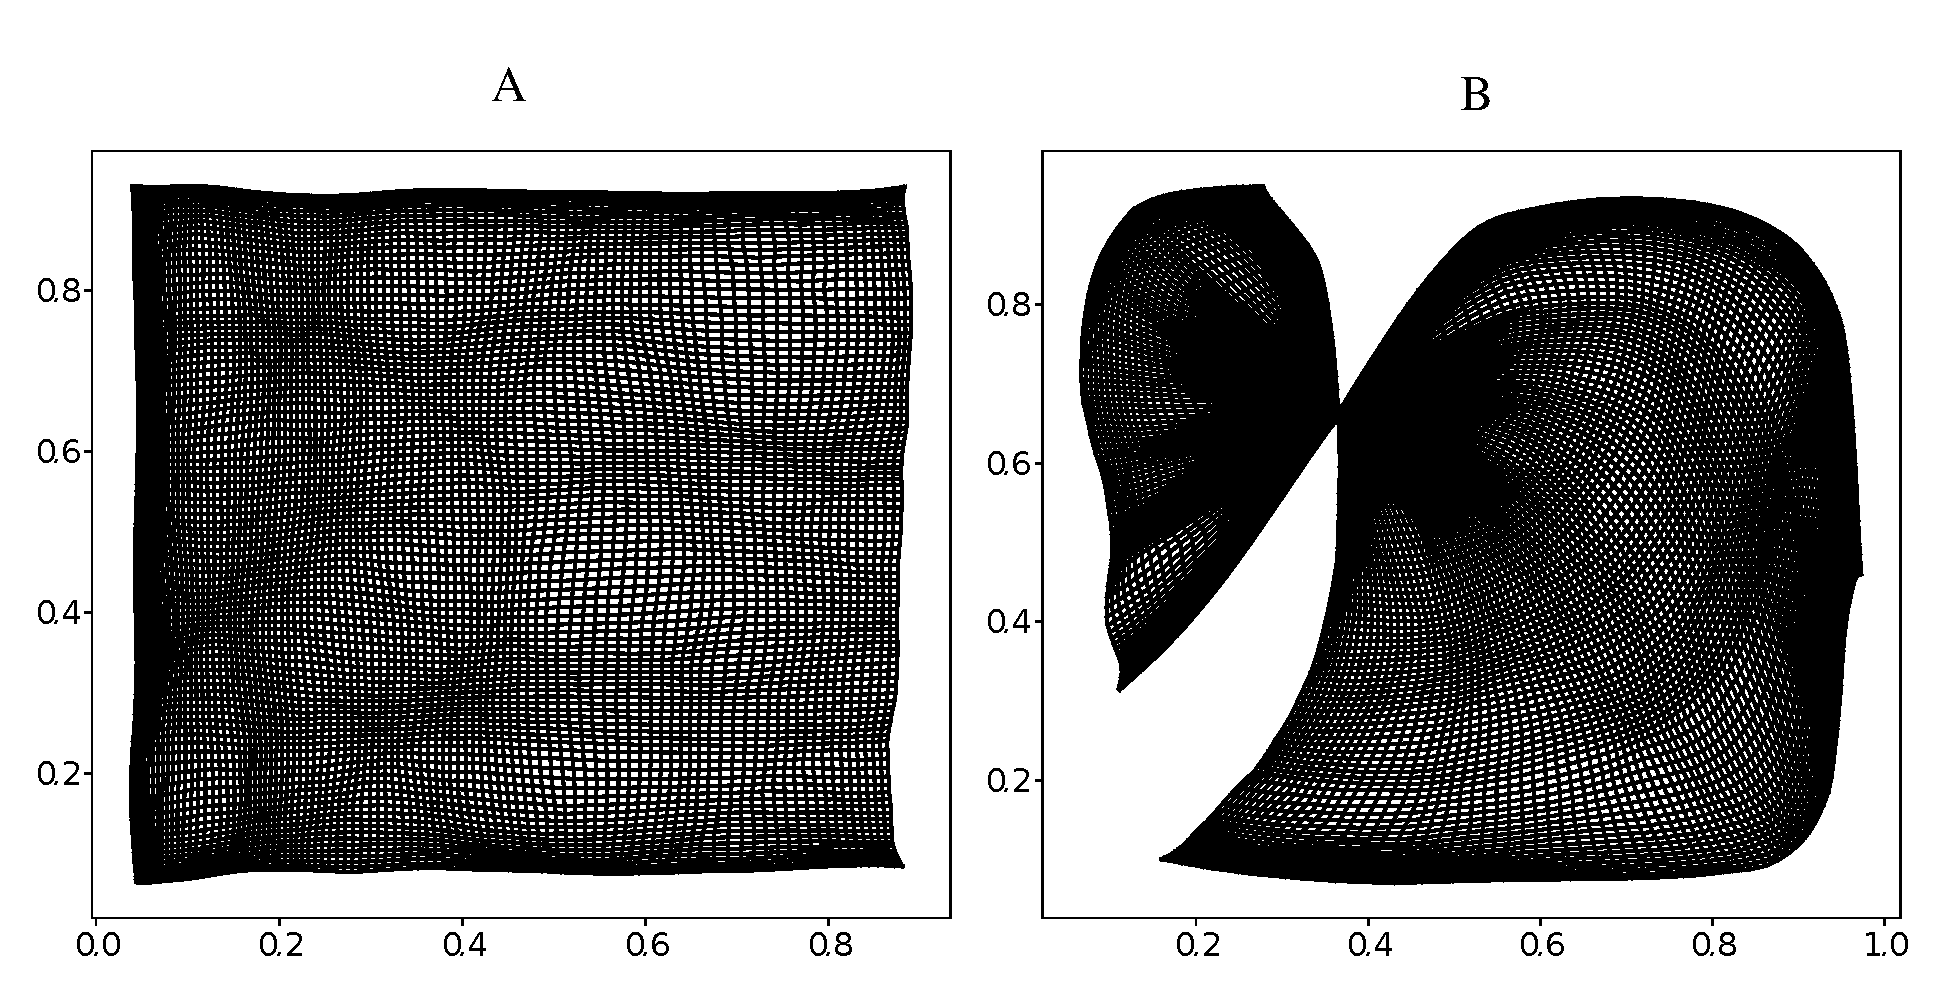
\includegraphics[width=0.6\textwidth]{we_cub_example.pdf}
		\label{fig:2som_cub_we}
	\end{minipage}
	\begin{minipage}{\textwidth}
		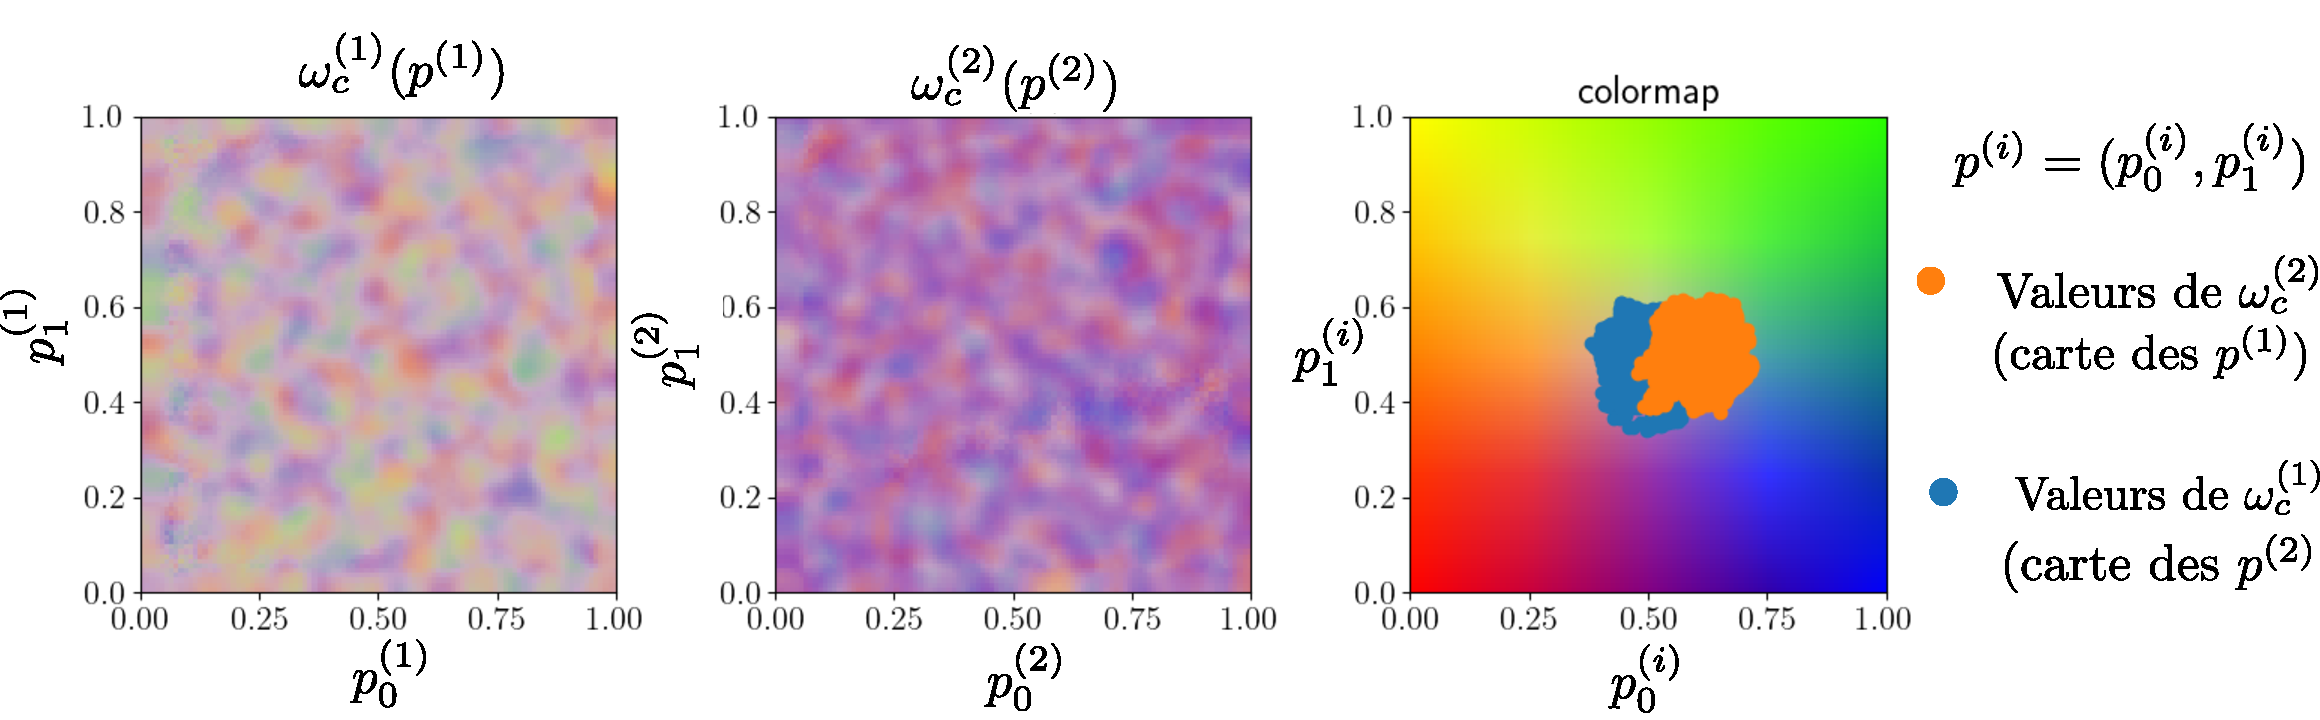
\includegraphics[width=\textwidth]{wc_cub_legend.pdf}
		\caption{En haut: poids externes des cartes $M\m{1}$ et $M\m{2}$ représentés sous forme de distorsion de la carte après 200000 itérations.
	En bas: poids contextuels des cartes pour la même itération, représentés sous forme de carte de couleur en deux dimensions. Un pixel situé à la position $p_i,p_j$ prend comme couleur correspondante la valeur 2D de son poids contextuel, associé à une couleur par la carte de coloration représentée à droite de la figure.
	Les points orange et bleus indiqués sur la carte de coloration sont les valeurs effectivement prises par toutes les valeurs de $\w_c^{(1)}$ et $\w_c^{(2)}$, cartographiant les positions des BMUs de l'autre carte.
	On remarque donc que les poids contextuels ne se déplient pas sur toutes les valeurs prises par les BMUS, car toutes les unités de la carte ont été BMU lors de cette phase de test.\label{fig:2som_cub_wc}}
	\end{minipage}
\end{figure}

\subsection{Organisation des cartes sur des entrées liées}

Nous avons vu que les cartes en deux dimensions font apparaître des motifs dans les poids contextuels tout comme en une dimension, mais que les poids contextuels ne peuvent pas se déplier si les données ont trop de degrés de liberté, faut de nombre de n\oe{}uds disponibles.

Nous étudions maintenant l'organisation des cartes sur des données pris sur une sphère 3D, tournée dans un espace en 4D. Les données ont ici deux degrés de liberté, représentées par les coordonnées polaires des points sur la sphère. 

La figure~\ref{fig:2som_s_002_wc} présente la disposition des cartes après 700 000 itérations d'apprentissage. 
Dans le cas présenté ici, les poids ont convergé vers une position stable~: seule la partie dans laquelle les motifs sont plus resserrés évolue encore après les 700000 itérations, mais sur un cycle limite. On peut donc dire ici que les poids ont convergé vers ce motif.
Les poids externes cartographient les entrées externes de la même façon qu'une carte indépendante, ce qui est bien attendu du modèle CxSOM. 
Nous observons ici la formation de motifs par les poids contextuels de la carte. Ces motifs rappellent bien les motifs présents en une dimension en faisant alterner des valeurs opposées (rouge et vert).

Le tracé des entrées en fonction de la position du BMU fait figurer l'existence ici encore de zones mortes.

Une première différence avec les cartes en une dimension est la forme des zones, moins régulières. Ces zones semblent dépendre des paramètres choisis. 
Dans une seconde expérience, nous avons pris $r_c = 0.05$ et $r_e = 0.2$, sur les mêmes données d'entrées. 
Nous remarquons que l'expérience 2 conduit à une configuration stable des poids contextuels, dont certains ont convergé vers un point fixe et d'autres vers un cycle limite. 
Enfin, la figure \ref{fig:wc_003} présente l'évolution des poids contextuels pour $r_c = 0.03 et r_e = 0.2$. 

Nous observons cependant une organisation commune à ces trois expériences, ce qui montre que les motifs dépendent bien de la relation entre entrées et non des conditions initiales des expériences. Les poids contextuels tendent à s'organiser sous une forme hélicoïdale, formant les motifs observé dans les trois expériences. 
Cependant, dans le cas ou $r_c = 0.05$, ce motif n'est pas un état stable et continue d'évoluer, les poids contextuels ne convergent donc pas.
Les poids externes, sur toutes les expériences, atteignent rapidement un état stable.

Nous pouvons conclure de ces observations préliminaires en deux dimensions que la formation de zones est un mécanisme qu'on retrouve dans des cartes 1D comme des cartes 2D. Cependant, les deux dimensions apportent beaucoup moins de contraintes sur la forme des zones que sur des cartes en une dimension, rendant possible la formation différents motifs sur les poids contextuels. 
Contrairement au cas en une dimension dans lequel la convergence des poids était assurée, la convergence des poids contextuels dans une carte 2D n'est pas assurée en fonction des paramètres de la carte. Cette étude paramétrique en deux dimensions apparaît comme une suite nécessaire de l'étude des cartes.

Nous avons analysé la forme des poids sur un seul type de distribution, une sphère dans un espace 4D, pour différents rayons de voisinage de la carte.
Nous observons que les motifs formés par les poids contextuels sont similaires dans tous ces cas et ne dépendent donc pas des conditions initiales des expériences: les poids des cartes sont initialisés aléatoirement de façon différente dans chaque expérience et les entrées sont tirées sur une même distribution mais de façon aléatoire.
Nous pouvons donc supposer que le type de relation entre entrées influence ces motifs. L'étude des comportements d'une carte 2D en fonction des entrées est une suite pertinente de ces résultats préliminaires.



\begin{figure}
	\begin{minipage}{\textwidth}
		\centering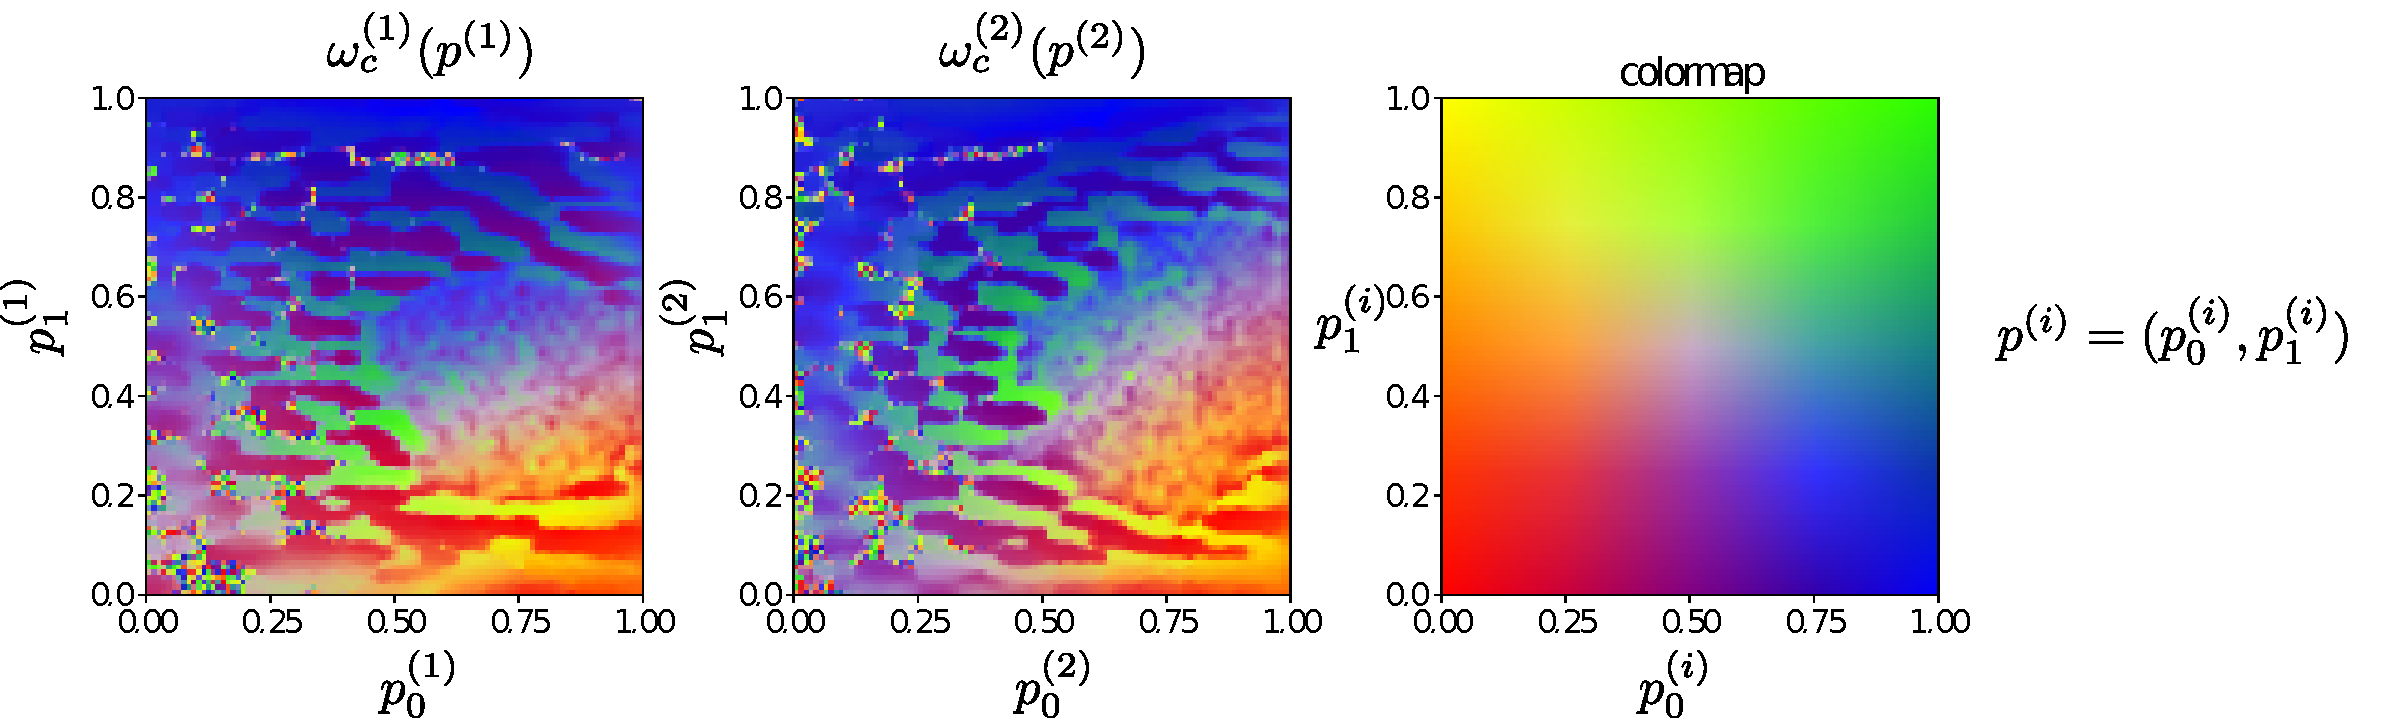
\includegraphics[width=0.7\textwidth]{wc_s_002_legend.pdf}
		\label{fig:2som_s_we}
	\end{minipage}
	\begin{minipage}{\textwidth}
		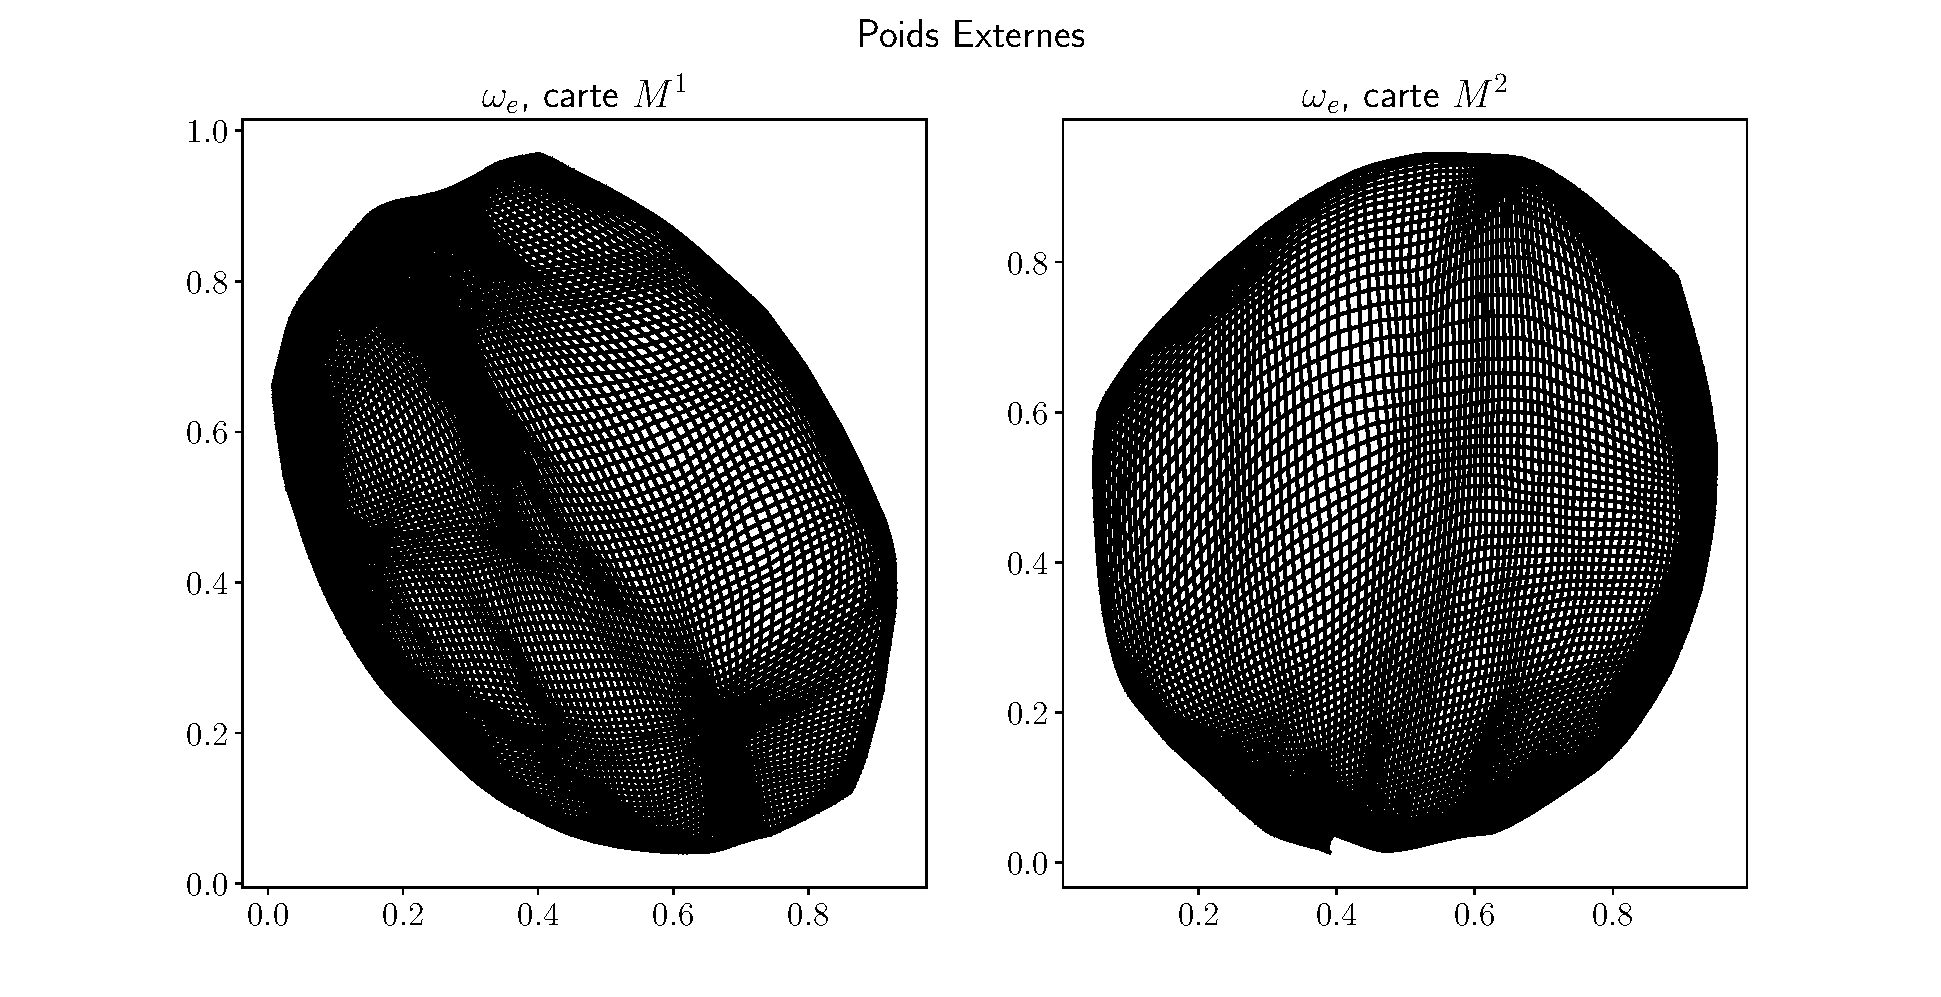
\includegraphics[width=\textwidth]{2SOM_sphere_we_249999.pdf}
		\caption{Tracé des poids contextuels d'une architecture de cartes, organisées sur une sphère dans un espace 4D, avec $r_e =0.2$ et $r_c = 0.02$. Contrairement au cas avec $r_c = 0.05$ précédemment tracé, les poids contextuels atteignent un état stable~: ils sont fixes dans toute la carte et sont dans un cycle limite dans la "tâche". Les motifs ne sont donc pas déterminés par les poids mais plutôt par les conditions initiales et l'évolution de la carte. Nous remarquons que les valeurs de $\w_c$ dans chaque carte se déplient bien ici sur toutes les valeurs prises par les BMU.
		\label{fig:2som_s_002_wc}}
	\end{minipage}
\end{figure}


\begin{figure}
	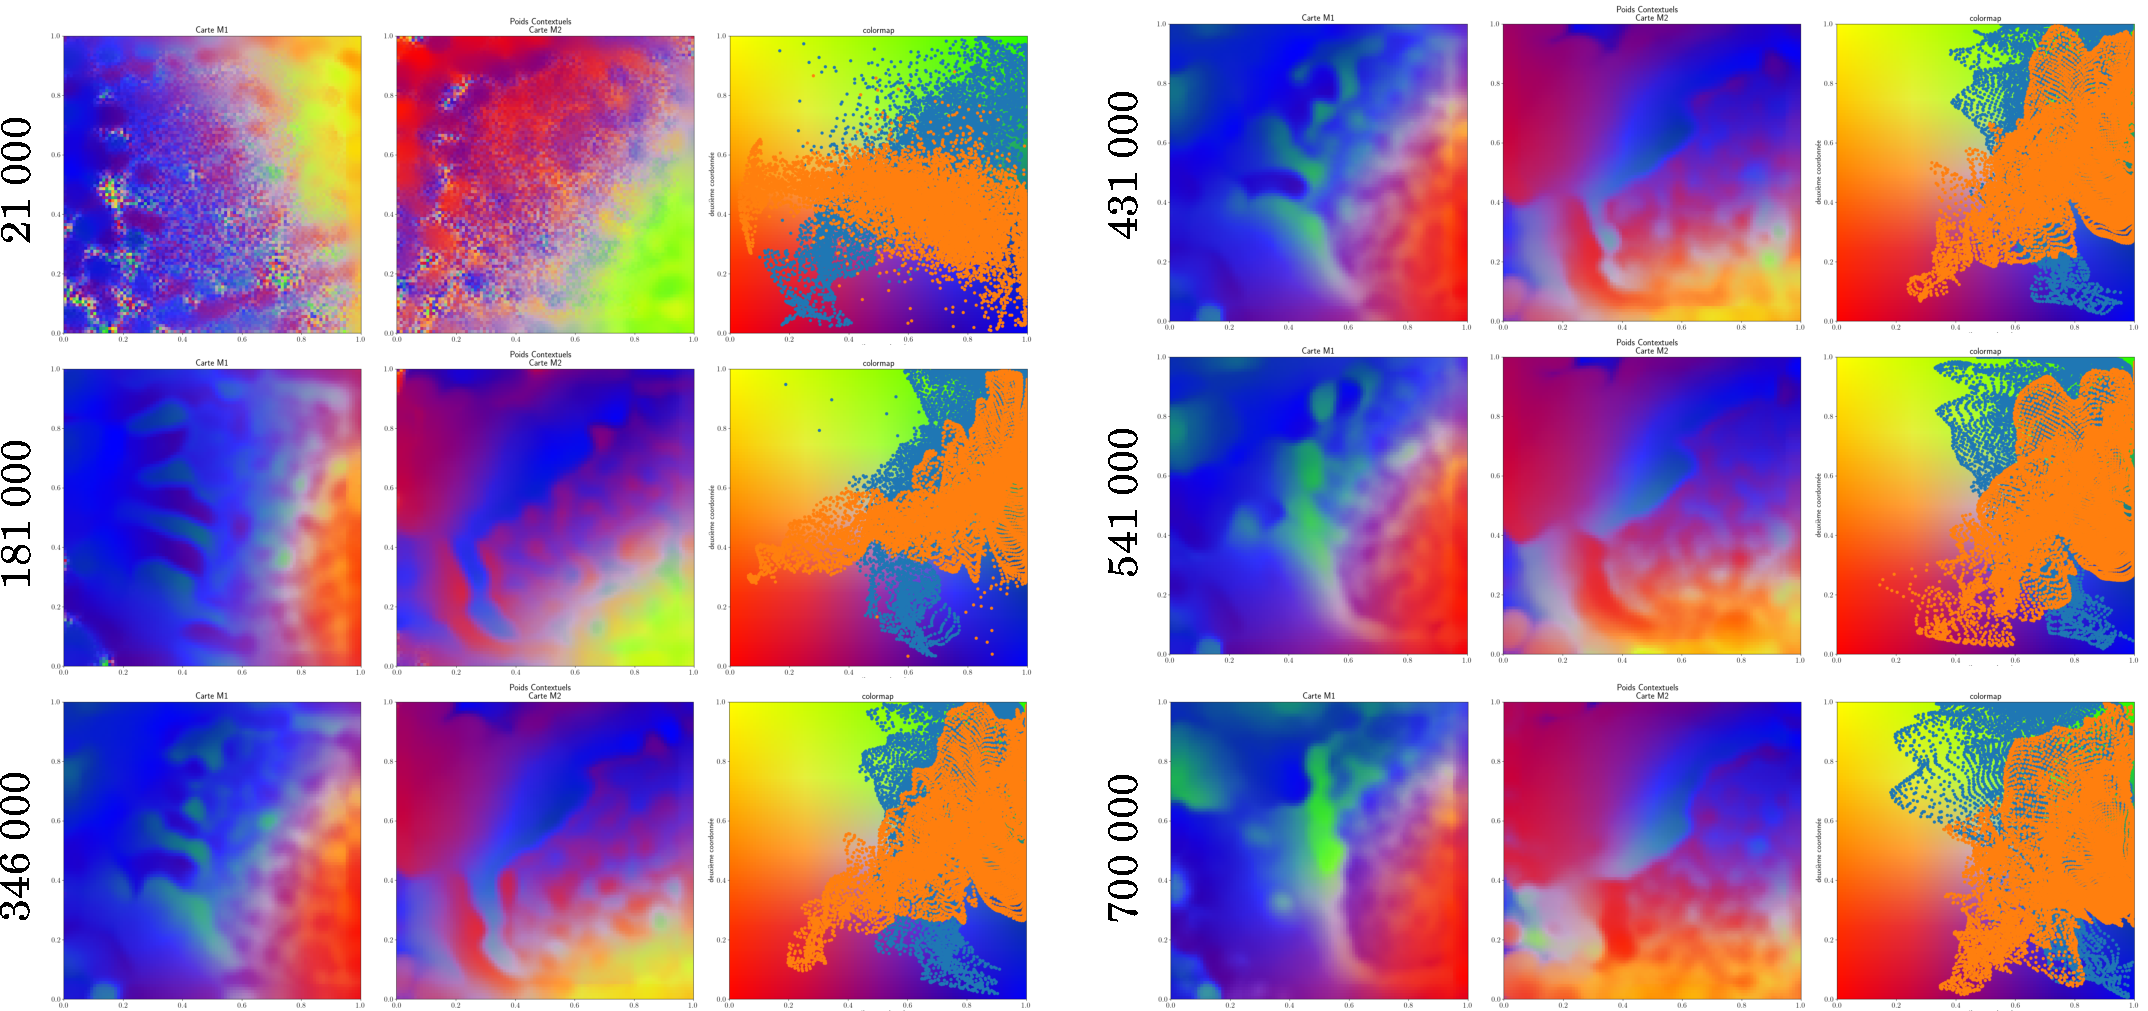
\includegraphics[width=\textwidth]{sphere_rc005_evol_landscape}
	\caption{Evolution des poids contextuels d'une architecture de deux cartes pour $r_c =0.05$. Les points sont représentés sous forme de carte de coloration à gauche et sous forme de disposition dans l'espace des positions sur la figure de droite. On observe une évolution régulière sous forme de motif en hélice, mais cette disposition évolue dans le temps. Après 700000 itérations, la figure semble se déformer vers de nouveaux motifs. Cette organisation ne converge pas.}
\end{figure}


\begin{figure}
	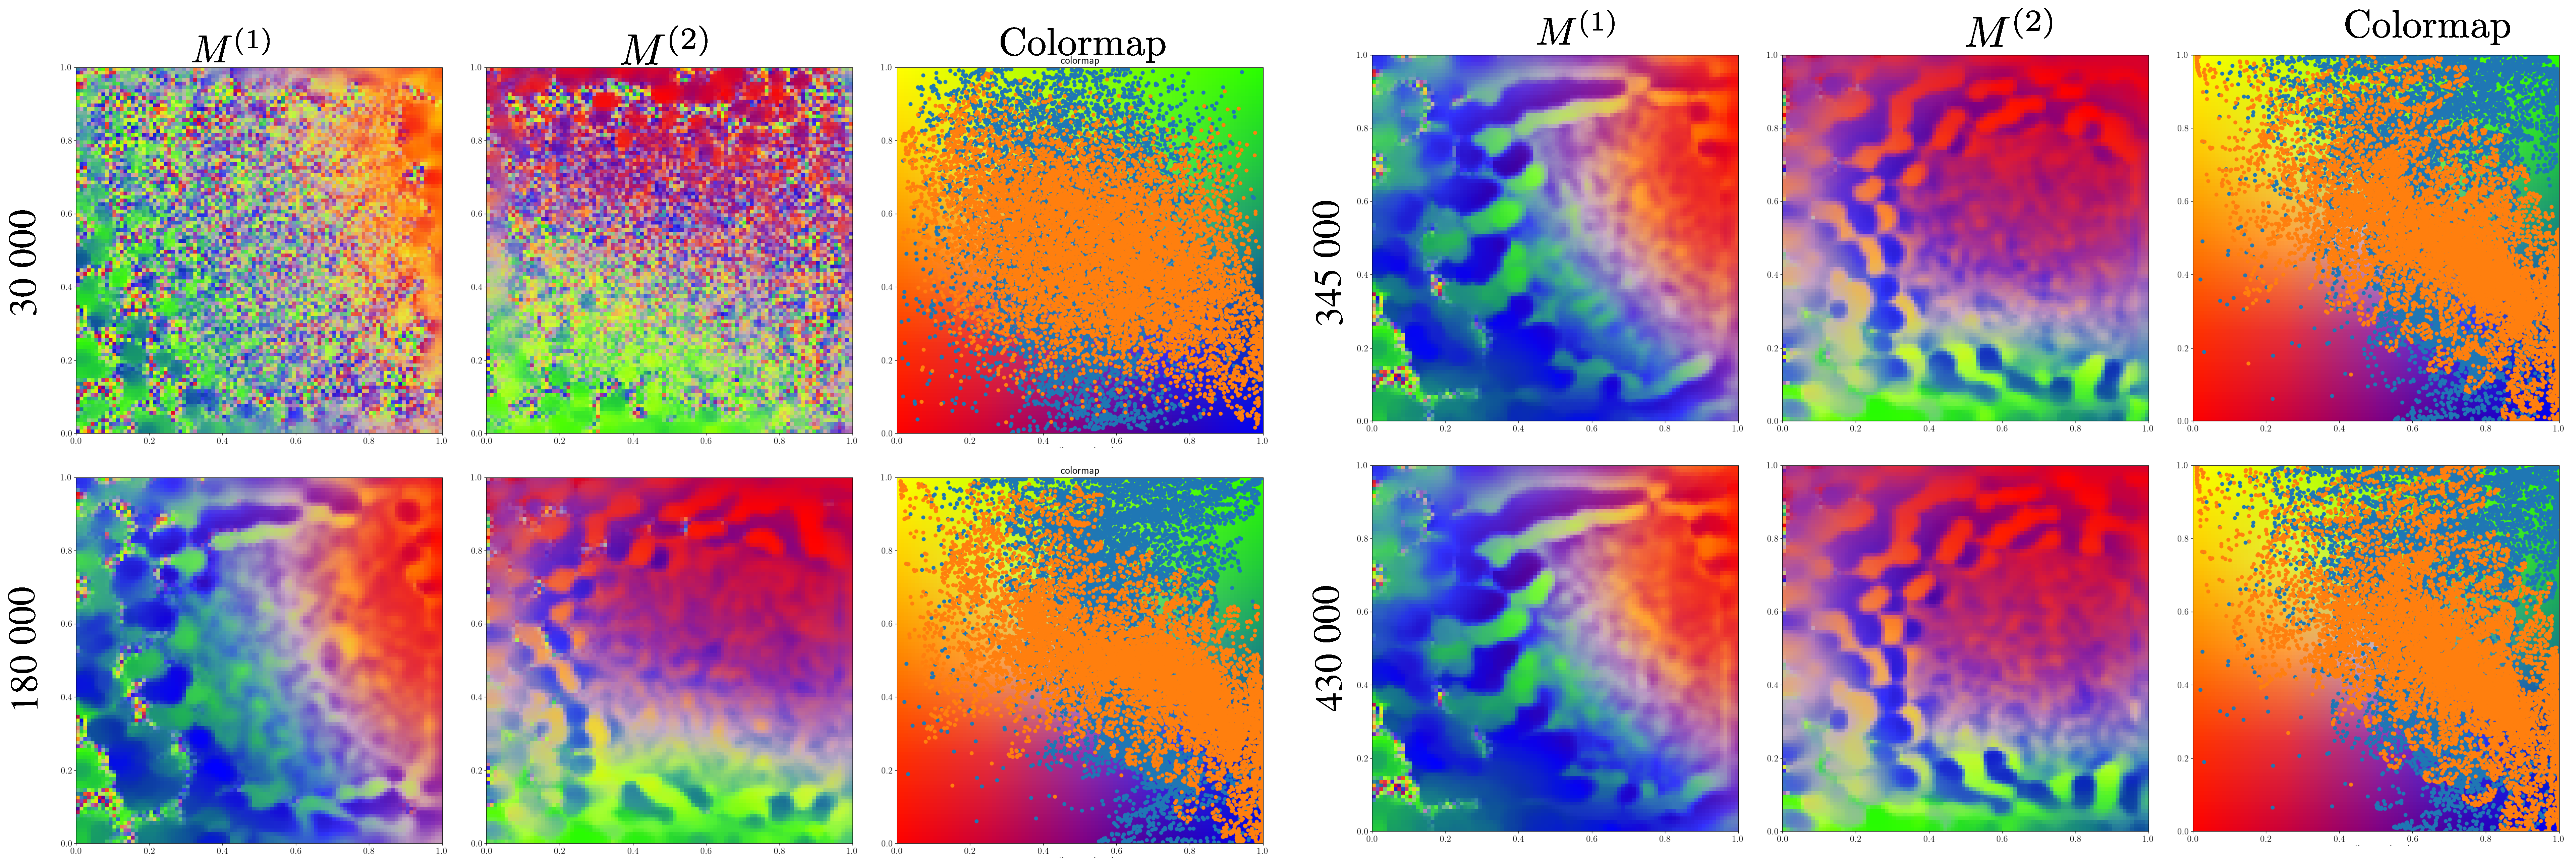
\includegraphics[width=\textwidth]{wc_rc003_evol.pdf}
	\caption{\'Evolution des poids contextuels d'une architecture de deux cartes pour $r_c =0.03$. Les motifs observés sont similaires à ceux observés pour d'autres paramètres. Les poids présentent toujours une forme hélicoïdale évoluant dans le temps.}
\end{figure}


%CONVERGENCE RELAX ! 

\section{Convergence de la relaxation}

Nous traçons enfin en figure TODO l'évolution du taux de convergence des tests au cours de l'apprentissage pour des structures de 2 et 3 cartes 2D en suivant le processus décrit au chapitre \ref{chap:relax}
Nous voyons que la relaxation converge bien y compris sur les cartes en deux dimensions.

Cette observation est prometteuse pour la construction d'architectures.

\section{Prédiction d'entrée}

Nous avons vu que les cartes en deux dimensions s'organisent, comme en 1D, de manière à former des zones dans les poids contextuels. Nous avons également observé que la recherche de BMU a un sens car la relaxation converge en fin d'apprentissage.
Nous nous attendons donc à ce qu'une architecture de cartes 2D soit en mesure de générer une prédiction.

Pour cela, nous construisons une architecture de trois cartes en deux dimensions prenant chacune une paire de coordonnées d'entrées en 6D. Ces entrées sont situées sur une sphère de dimension 3 plongée dans l'espace en 6D. $U$ est ici une variable $2D$. Dans cette configuration, la connaissance de deux entrées sur trois et du modèle permet de déterminer la troisième.

En figures~\ref{fig:3som_w}, nous traçons les poids externes et contextuels des trois cartes.
Nous remarquons également la présence de motifs dans l'organisation des poids contextuels.
Nous lançons une étape de prédiction à la fin de l'apprentissage lors de laquelle la carte $M\m{1}$ ne reçoit plus d'entrée externe. La valeur de $\w\ext\m{1}(\bmu\m{1})$ est alors utilisée comme prédiction de l'entrée $\inpx\m{1}$.
La Figure~\ref{fig:3som_pred} présente la valeur prédite en fonction de l'entrée $\inpx\m{1}$. Les valeurs étant 2D, nous traçons la courbe sur chaque dimension. 
Les tracés montrent que la prédiction est bien réalisée. Cela nous permet de conclure que la relaxation conduit bien à un BMU correspondant à la valeur de l'entrée, y compris en deux dimensions. Les tracés des cartes $M\m{2} et M\m{3}$ indiquent que les BMUs des autres cartes ne sont pas perturbés par le fait qu'il manque une entrée $\inpx\m{1}$.
Enfin, nous remarquons que cette erreur est plus faible que l'erreur observée sur une entrée  pour une architecture de 6 cartes 1D.

\begin{figure}
	\begin{minipage}{\textwidth}
		\centering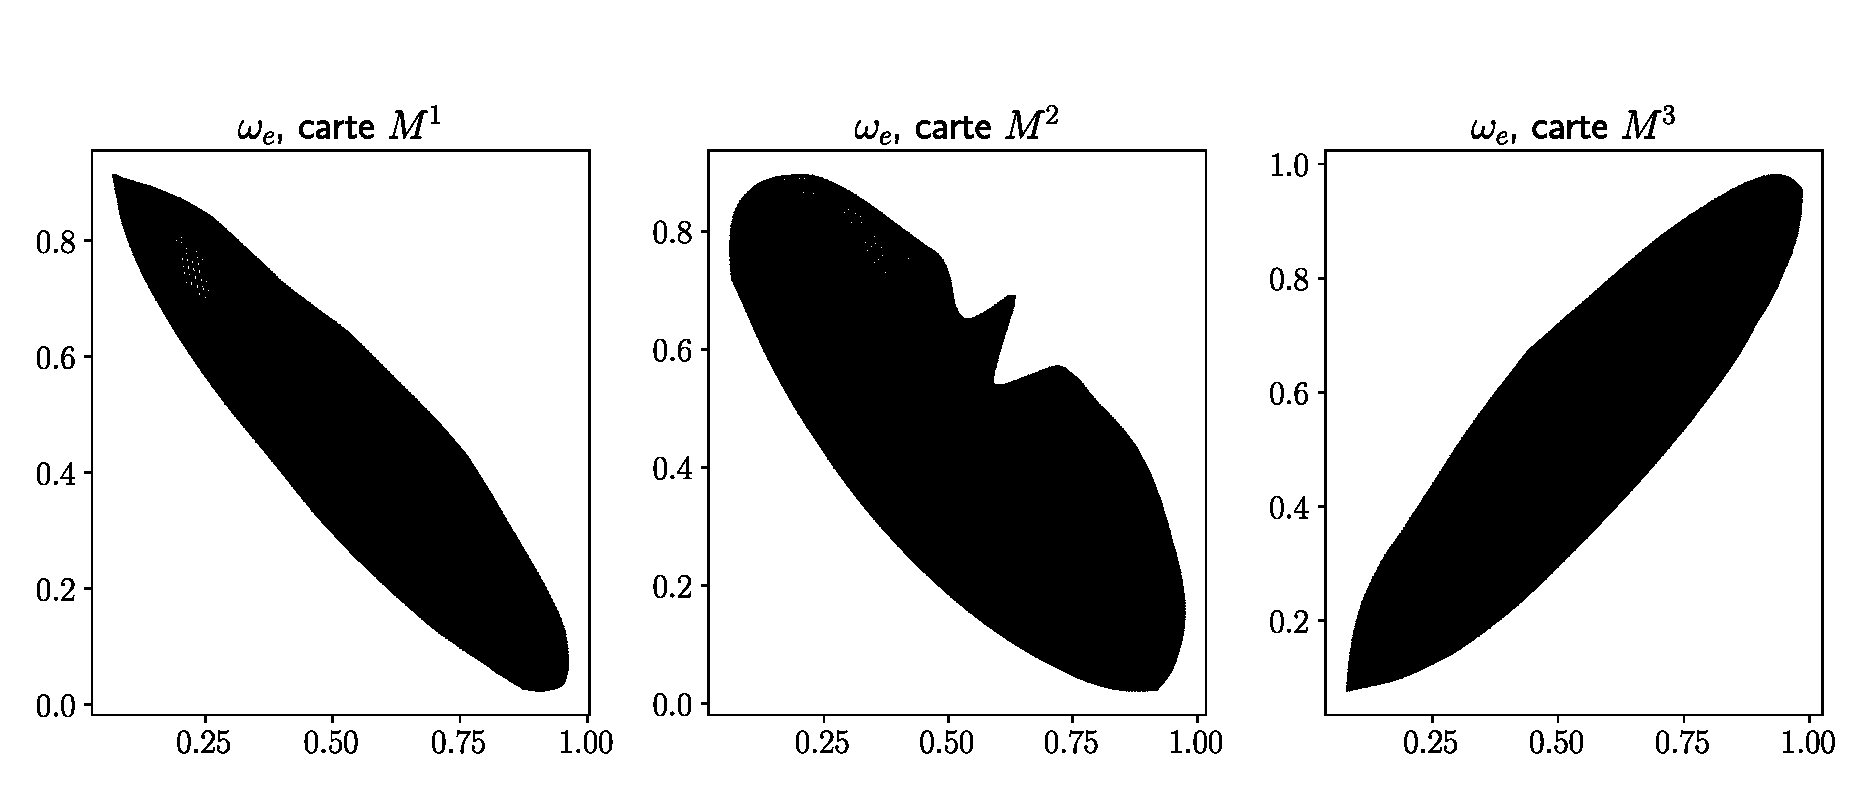
\includegraphics[width=0.7\textwidth]{3SOM_S_we_239999.pdf}
	\end{minipage}
	\begin{minipage}{\textwidth}
		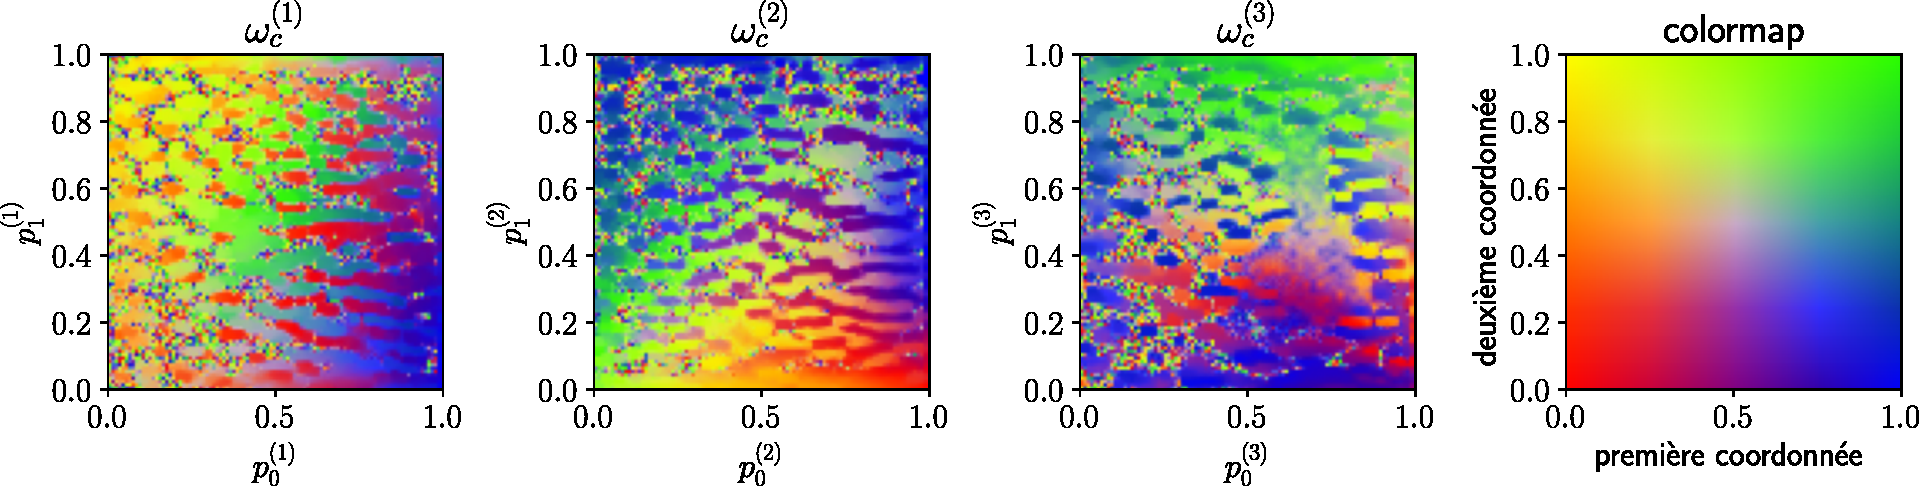
\includegraphics[width=\textwidth]{3SOM_S_wc_239999.pdf}
		\caption{\label{fig:3som_w}}
	\end{minipage}
\end{figure}

\begin{figure}
\includegraphics[width=0.7\textwidth]{zclosed-1-239999_error.pdf}
\caption{Tracé de l'erreur de prédiction $\w_e\m{1}(X\m{1})$ en fonction de la valeur théorique de $X^{(1)}$, non présentée à l'architecture, dans une architecture de trois cartes 2D prenant des entrées $X^{(i)}$ en deux dimensions $[X^{(i)}_0, X^{(i)}_1]$. Nous traçons sur une ligne, pour chaque entrée, les dépendances entre chacune des dimensions.
Lorsque la carte $M^{(1)}$ ne reçoit pas d'entrée externe. Les cartes $M^{(2)}$ et $M^{(3)}$ ayant une activité externe, le graphique montre que la quantification vectorielle est bien réalisée dans ces cartes. La carte $M^{(1)}$ est uniquement activée par les connexions contextuelles venant de $M^{(2)}$ et $M^{(3)}$. La figure du haut montre que la prédiction est correctement réalisée.\label{fig:3som_pred}}
\end{figure}

\subsection{Limites et perspectives}



%Convergence des cartes 2D Cottrell 


\ifSubfilesClassLoaded{
    \printbibliography
    %\externaldocument{../main.tex}   
}{}
\end{document}



% PLAN


% Convergence des poids :
% - Dépend des paramètres, contrairement à la carte en 1D on n'arrive pas forcément dans une position stable
% - Rc = 0.02 : point fixe, avec une partie 
% - Chaque expérience différente : grande dépendance aux conditions initiales. 